\documentclass[border=10pt]{standalone}
\usepackage{tikz}
\usetikzlibrary{decorations.pathmorphing,patterns}
\begin{document}
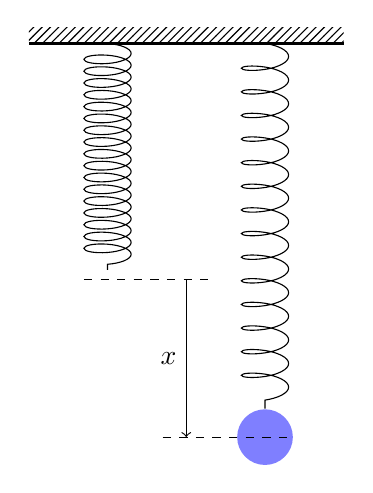
\begin{tikzpicture}
  \node[circle,fill=blue,inner sep=2.5mm, opacity=0.5] (a) at (2,0) {};
  \node [] (b) at (0,2) {};
  \draw[decoration={aspect=0.3, segment length=3mm, amplitude=3mm,coil},decorate] (2,5) -- (a);
  \draw[decoration={aspect=0.3, segment length=1.5mm, amplitude=3mm,coil},decorate] (0,5) -- (b);

  \draw [->] (1,2) -- (1,0) node [midway, left]{$x$};
  \draw [dashed] (-0.3,2) -- (1.3,2);
  \draw [dashed] (0.7,0) -- (2.3,0);
  \fill [pattern = north east lines] (-1,5) rectangle (3,5.2);
  \draw[thick] (-1,5) -- (3,5);
\end{tikzpicture}
\end{document}
